%%% mode: latex
%%% TeX-master: t
%%% End:

\chapter{绪论}
\label{cha:intro}

硕士学位论文应能表明作者确已在本门学科上掌握了坚实的基础理论和系统的专门知识,并对所研究课题有新的见解,有从事科学研究工作或独立担负专门技术工作的能力。硕士学位论文的字数一般不少于2.5万字,加上各类图表,从绪论到总结与展望的总页数一般不少于65页。否则,可能显得工作量不够饱满。

学位论文题名是以最恰当、最简明的词语反映论文中最重要的特定内容的逻辑组合。题名既要准确地描述内容,又要尽可能地精练,一般不宜超过30个字。题名一般避免使用不常见的缩略词、字符、代号和公式等。若实属必要,需要摘要中给出中英文全称与缩写。学位论文内容应结构合理、立论正确、推理严谨、文字简练、层次分明、逻辑严密、数据真实可靠。

学位论文文字排版的字号、行距、字距的大小,以版面清晰、容易辨识和阅读为原则。为统一起见,具体要求如下:
\begin{enumerate}
    \item[(1)] 论文页眉,楷体,小二
    \item[(2)] 章和节的题名用黑体,字号分别用三号和四号
    \item[(3)] 正文内容用宋体,英文用Times New Roman,小四号;行间距1.5倍;正文注意两侧对齐
\end{enumerate}

绪论部分是整篇论文的导引,应包括选题背景、意义;国内外研究概况;前人研究中存在的问题或知识空白;进而引出本文的研究设想,简要给出全文各章节的主要内容、以及章节之间相互联系。

在写作中无论是研究背景及意义,还是国内外研究现状,要做到有依据都必须引用参考文献。通常情况下,绪论部分的参考文献应占全文参考文献的百分之80以上。参考文献的顺序必须是按照在文章中出现的先后顺序进行排列。

以下简要说明一下绪论部分的内容及各级标题格式等。


\section{研究背景与意义}
\label{sec:general intro}
主要介绍与本文相关的基础知识,包括基本概念、理论、原理、方法与技术等,指出相关领域研究工作的意义。

在写作上要深入浅出,图文并茂,以便大同行也能读懂。

\subsection{**概念}

\subsection{**技术}
...

\section{XXX国内外研究现状(请拟定具体的题目)}
\label{sec:requirement}
此处应就与本文相关的国内外研究概况进行全面综述,这样相关内容在后面章节中就可以点到为止,无需再大段大段地分别介绍了。



\section{存在的问题}
\label{sec:compile}

综合当前国内外研究现状,总结现有研究中存在的问题,以便引出本文的研究内容。

在绪论中提出问题,论文的工作正是围绕这些问题而展开。


\section{本文主要内容}
\label{sec:checklist}

不同学生学位论文的类别各异,大致可分为工程类,理论类、算法研究类、仪器/工艺设计与研发类、综合类等。不同论文的章节结构各异,但每种类型的论文还是有其特定的格式。原则上,硕士论文的主体研究内容不得少于2章,加上绪论 、总结与展望,累计不得少于5章。

作为华中科技大学硕士学位论文模板,本文首先给出了不同类型的研究论文典型结构供大家参考,再根据学术出版的规范化要求,说明论文写作中的细则。全文共分为5章。主要内容如下:

第一章 绪论:简要介绍论文的研究背景、国内外研究现状、存在的问题,给出全文的主要研究内容。为了让读者更容易理解全文,建议用一个文档结构图给出各章节逻辑关系。

本文共分为5章内容,章节内容之间的关系图如图~\ref{Fig1-1}所示。

\begin{figure}[!htbp]
    \centering
    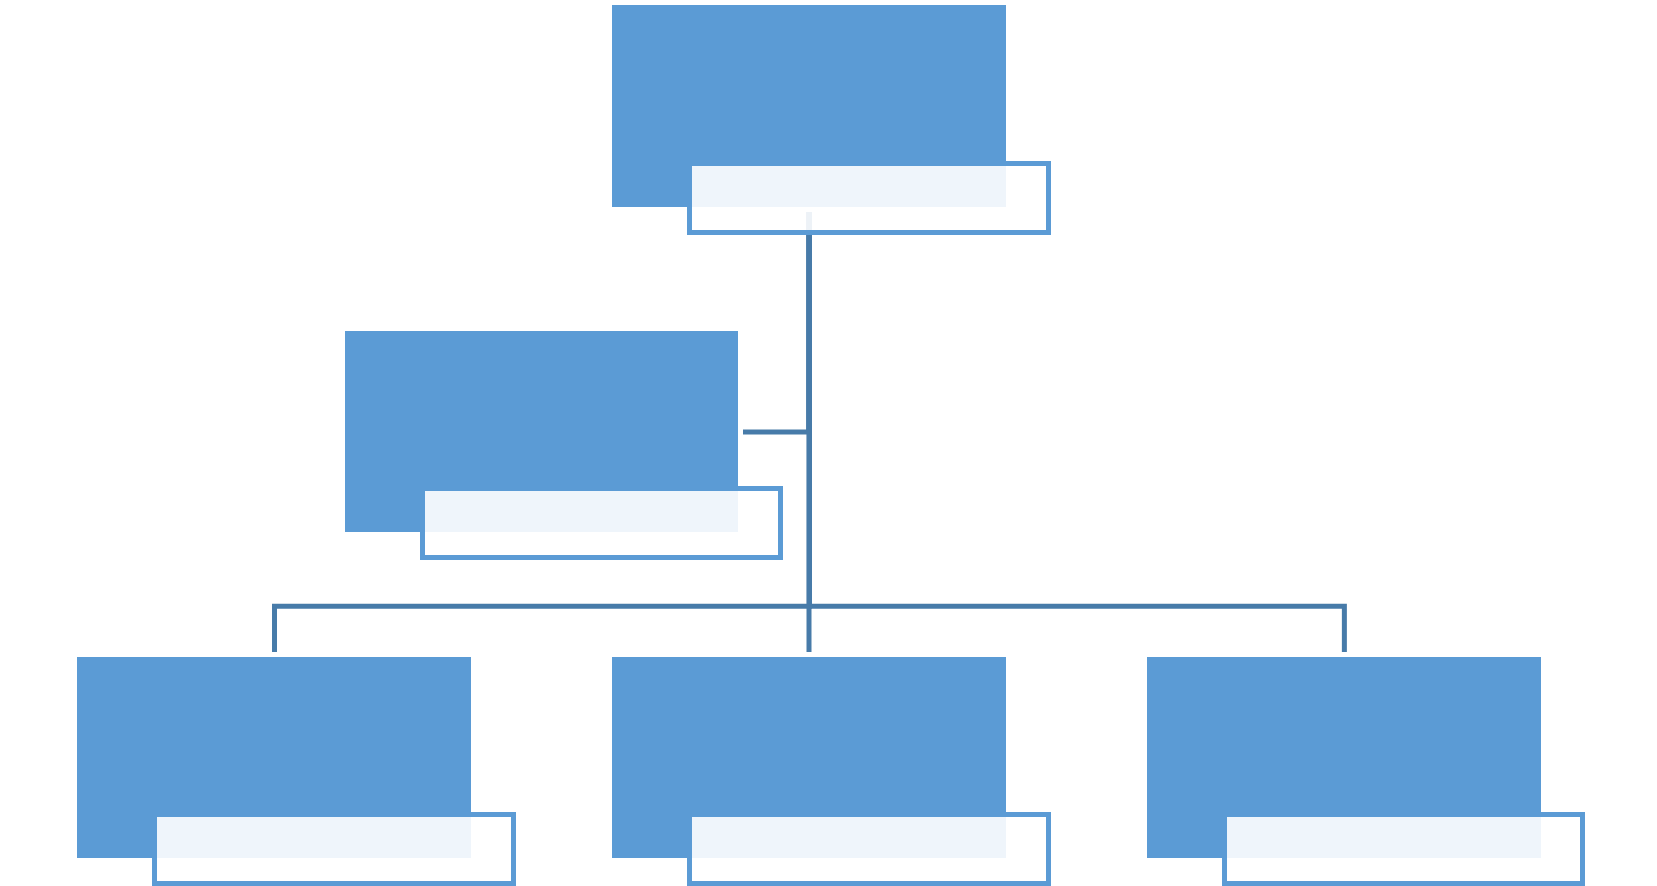
\includegraphics{figures/Fig1-1.png}
    \caption{组织结构图}\label{Fig1-1}
\end{figure}

第二章 系统与控制理论类论文结构:……

第三章 算法研究类结构:……

第四章 学位论文写作细则:……

第五章 总结与展望:给出全文的主要内容及结论,总结本文的创新点,并对未来的工作进行展望。

